\section{Prerequisite Concepts}

Like many other domains, within the study of robotics, path planning involves the understanding and implementation of concepts borrowed from other disciplines. This section attempts to present key concepts and details in hopes of anchoring the following discussion about path planners by first contextualizing some of the important tasks, principles, and assumptions that are fundamental in the design and implementation of the several planners covered in this paper. 

% \subection{Workspace, Task, Configuration Space}

\subsection{Maps \& Mapping}

One of the most fundamental requirements for any path planning system is to develop an understanding of where it is in the physical world. It would be impossible for a robot to navigate its environment without ability to know where it currently is and what its final destination or goal state is. This implies a need for a robot to generate a representation of its environment which it can use to solve its problems. 

By definition, a physical environment is the ground truth representation which we would like the robot to understand; however, this is typically impossible because of intrinsic limitations. The best that we can do is to embed as much information as possible about the physical world into a simplified representation. This is known as mapping.  

Mapping is the process of extracting useful features or landmarks, from within an environment, and structuring these features into a, compressed and lossy representation/idealization generated from the original environment. These representations can be anything from dense 2D/3D lidar point clouds to abstract features; however, one of the primary tradeoffs when generating a map is the balancing of simplicity, size, and data quality. More often than not, maps are chosen to be as simple as possible while attempting to preserve feature quality (e.g limit uncertainty), in a way that is still capable of solving the problem at hand.  

Finally, the representation we use in a map has a tremendous impact on the fundamental design and limitations concerning how a path planner functions. Additionally, the concept of map generation is closely tied to the topics of sensing and localization, in the topic of SLAM, which is itself a very in-depth sub-field of robotics. \linebreak  

\subsubsection{Dimensionality Reduction \& Discretization}

In the era of computers, map generation routinely tradeoffs quality and quantity of information for portability and efficient access by a computer. This typically means that maps must be compact enough to fit into memory. Even though robots exist in a three-dimensions of space, it is often sufficient to navigate the 3D world, by planning a path in a 2D projection. This technique is called \textbf{dimensionality reduction}. 

Unfortunately, even a 2D continuous map is often computationally untractable, with modern computers. The most common solution for this problem, not just in robotics but also in numerical methods, is to discretize the continuous domain into discrete grids or cells. By doing so, the computer can efficiently store and query a map in RAM. The side-effect of discretization is an unavoidable loss/degradation of the original information.  


While undesirable, carefully parameterization and clever discretization methods aid in mitigating lossy behavior, or ensure that any degradation of quality is functionally insignificant to the problem at hand. There are several popular discretization schemes, with the most common listed below. 

\begin{itemize}
  \item Uniform Grid
  \item Quad Tree (2D discretization)
  \item Oct Tree (3D voxelization)
  \item Delaunay Triangulation (2D or 2D Mesh generation)
\end{itemize}


Generally, the most commonly used method is a uniform discretization. This structure is intuitive, simple to understand, and fast to implement in code; however, uniform discretization is subject to the curse of dimensionality. Whenever an environment is large and requires a high resolution, uniform grids become slow to search and expensive to store. In these situations, a clever trick is to partion a space into an non-uniform grid structure using Quad or Oct trees. These data structures are built so that they will keep the grid as large as possible unless it is a region of the map that is determined to require higher resolution. 

% \subsubsection{Inverse Sensor Model}

% One of the most important parts of the mapping process is the generation of map features from global knowledge or sensor data. 

% Given a uniformly discretized mapping, we still need to 

% % Now that we have talked about what a grip map is, why they are important and how they are used in mobile robotics, talk aobut how we can use a 2d Planar lidar to create one using the inverse sensor model. 
% % \subsubsection{Bresenham Line Algorithm}
% % Then... Discuss how due to the nature of the grip map being discretized we need a method to deterine which pixels should be included to create a straight line. 
% % Discretization causes aliasing (jagged edges) bresehams line algorithm allows use to draw a line between any two pixels on a screen. (used in computer graphics)
% % For grid map generation, we used bresehams line algorithm as a model of the laser beam to determine which cells of the grid map are free space and which cells are occupied. 

% There are a limited number of situations that violate this assumption; however, these counter-examples typically rely on the existance and ability to access \textbf{global} data about an environment. An common example of this occurs in video games or simulations where the position of a character, game object, or element is known \textit{a priori}. In this class of applications, a character/robot does not need to localize itself or sense its' environment, in the classical sense, as the entire world is a construction which can be queried. 


\subsubsection{SLAM}
Frequently, there exists situations where functional maps do not exist for a given environment, and they must be either preprocessed or computed on the fly by the robot as it traverses the environment. The latter operation is known as \textbf{Simultaneous Localization \& Mapping} or SLAM for short. SLAM is an incredibly detailed field of study with many different approaches from EKF SLAM, Graph SLAM, RGBD SLAM, and other vision based SLAM algorithms

For the purpose of this paper, it suffices to say that without a complete or partial mapping of the environment, the robot will first have to construction the map before its able to fully plan a path through the environment. While important, for the planners implemented in this paper, we assume that map has already been generated and has been provided to the path planner offline.

\subsubsection{Occupancy Grid Maps}

One of the most popular mapping representations is that of the \textbf{occupancy grid map} (OGM), also referred to as a probability grid map or PGM. As the name implies, this map is composed of a grid; however the unique distinction of an OGM is that it each grid is associated with a value (more specifically a probability) ranging from $[0, 1]$. This value indicates the probability that that grid cell is occupied. Zero indicates completely free and one indicated completely obstructed, with any value between indicating the likelihood of occupancy. 

One of the many advantages an occupancy grid map possesses is how computers store and process them. If we assume a 2D grid map with a uniform discretization, the grid map effectively becomes a grayscale picture of size $m \times n$pixels and a resolution of $2^d-1$, where "d" is the bit depth. The similarity between occupancy grid maps and grayscale images is so complete that most grid maps are actually stored as 8-bit grayscale images within the computer. This is very practical as many programming languages have libraries that can easily read in images and perform operations on them. The remainder of this paper assumes that every map is encoded as a occupancy grid map. 

% 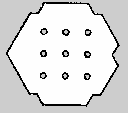
\includegraphics[scale=1]{map.png}

% \begin{wrapfigure}
%   \centering
%   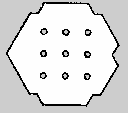
\includegraphics[width=.2\textwidth]{map.png}
%   \label{fig:Probablistic Grid Map}
%   \caption{Probablistic Grid Map}
% \end{wrapfigure}


\subsection{Graph Generation}
While not universally true, graph-based planners have historically been the most popular and practical implementation for defining non-trivial sized maps. For the purposes of this paper, all of the planners that we will cover are graph-based and use some variant graph-like datastructure (e.g. graphs or trees). 

\subsubsection{Grid World}
One of the most common approaches to constructing a graph is the notion of directly converting each cell of an occupancy grid map, and then applying rules for how to wire up the edges between each of these nodes. This is called a \textbf{grid world}. The uniform node generation and rule-based edge generation of this graph mean that this graph is intuitively very and extremely simple to implement programmatically.

The two most popular connectivity rules are known as \textbf{connected-8} and \textbf{connected-4}. In connected-4, the rules that we imposes on transitioning to a new cell limit legal moves to up/down/left/right (no diagonal motion is permitted.) while connected-8 graphs are allow to move 1 cell in any direction up/down/left/right and diagonals. In addition to these connectivity rules, there are two different methods concerning how obstacles can be integrated into the final graph. 

These two methods are \textbf{infinite edge weights} and \textbf{edge removal}. Infite edge weighting works by guaranteeing that the shortest (aka lowest cost) path through the graph will never be through an obstacle. Since transitioning to a node that is an obstacle will incur and infinite cost (as far as the planner is concerned), this mean prevents obstacles from being included in the final path. On the other hand, the edge removal method simply removes all edges that would connect to an obstacle node, in the graph. This method works by literally making it impossible for the planner to traverse obstacles as they have all been removed from the graph.

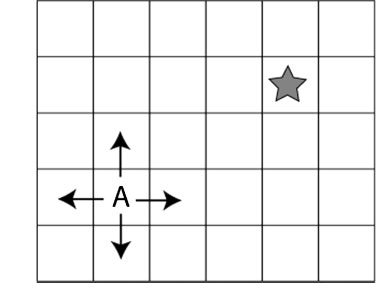
\includegraphics[scale=.23]{grid_world_pict.png}

% \begin{figure}[t]
%   \includegraphics[width=8cm]{Plot}
%   \centering
%   \label{fig:birds}
%   \end{figure}


% 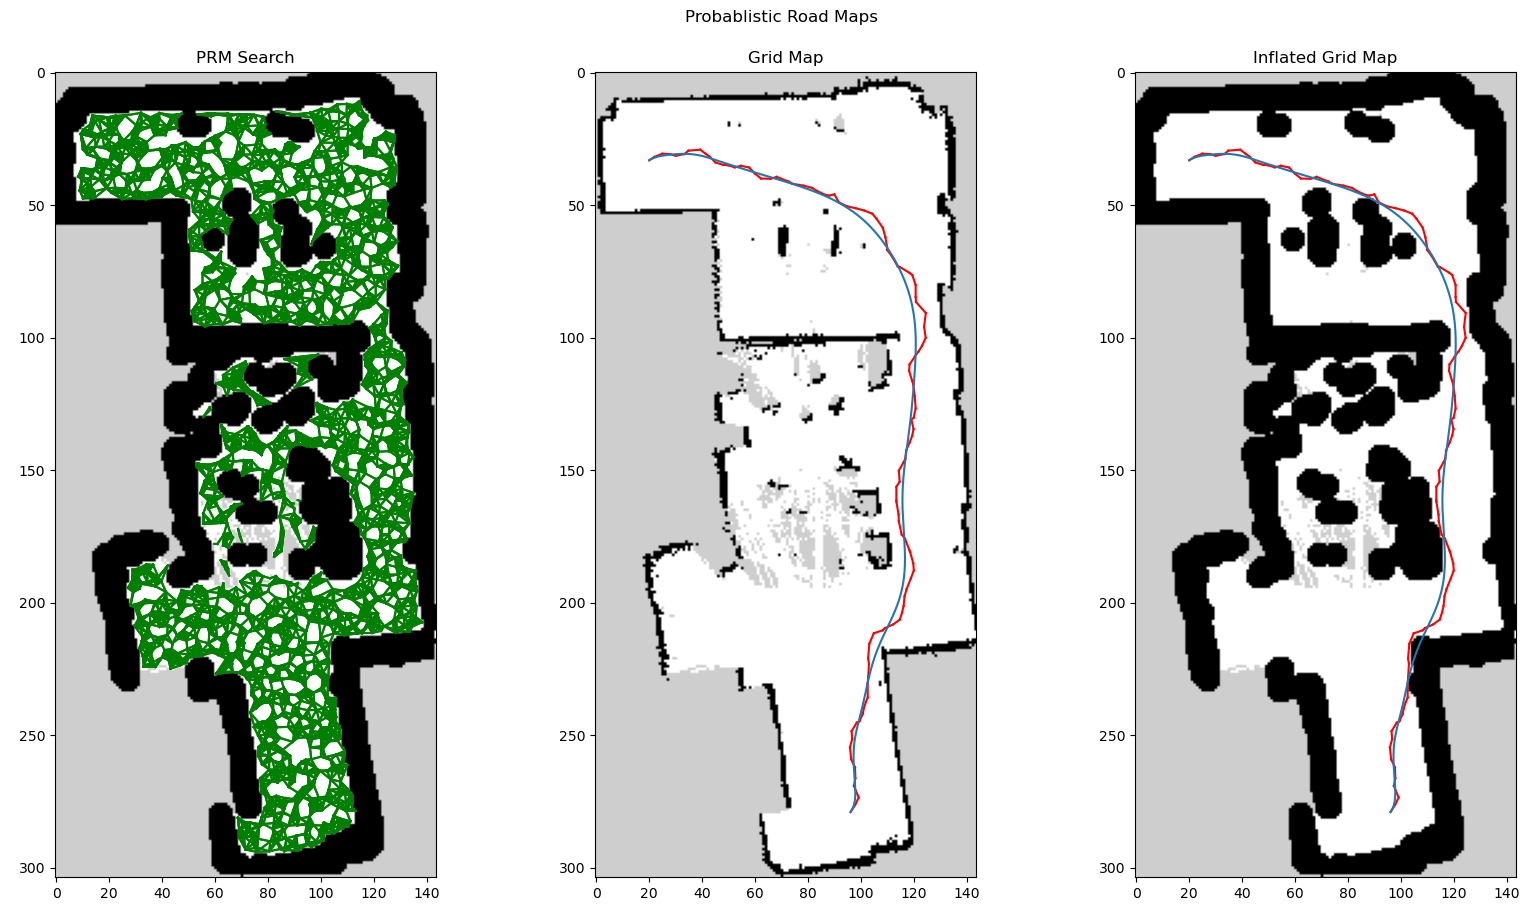
\includegraphics[scale=.23]{probablistic_road_map.png}


\subsubsection{Random Sampling}

One of the downsides of grid world search graphs is the node density. By definition, every pixel of the occupancy grid map could represent a free cell, and is subject to the curse of dimensionality as the size of the map increases. To address this scaling problem, a popular technique is to employ \textbf{random sampling}. This approach is based on the concept of Monte Carlo methods, where uniformly sampling map is used to create the nodes on the graph. 

In principle, in the limit as the number of samples approaches infinity, we can guarantee the convergence of our path planner to the globally optimal path (if it exists). In practice, sampling-based methods can possess an order of magnitude fewer nodes while still providing enough coverage at a high enough sample density to produce a feasible  path through the environment that is trending towards the global optimal path. An excellent example of this in shown the in probabilistic road maps algorithm. 

\subsubsection{Obstacle Inflation}

One of the pitfalls of using occupancy grid maps as the basis for the search graph is that each cell is effectively a pixel in an image. Depending on the density of our sensor coverage, there is a non-zero chance that paths through the environment that are only a single pixel wide exist. This is a problem for our robot if it happens to be larger than the adjusted realworld scale of the pixel. This is almost always the case. 

To prevent situations like this from occurring and generating paths through infeasible regions of the map, we can apply a technique known as an obstacle inflation. This very simple technique artificially scales up every obstacle pixel in the scene take up more space than the actual sensor reading indicated. The result of this \textbf{inflation} is that sensor noise is usually absorbed into these inflated obstacles. Additionally, this technique provides a sort of poor-mans approach to prevent the phenomenon of "wall-hugging". In simple implementations of path planner, the planner does not have a concept of "robot size". This means that the planner will attempt to make the shortest path between two points, even if it that path is infeasible for the robot to traverse. This is demonstrated as a sort of type of behavior where the path generated hugs walls in the environment to attempt reduce the distance (total cost) of the path. By applying an appropriately sized inflation layer, we can guarantee that the path between points, accounts for the physical footprint of the robot. While nifty, there are more sophisticated techniques based on applying cost gradients as a function of the distance away from an obstacle/wall. The cost gradient incentivizes the planner to prefer cells that are farther away from walls; however, this requires more postprocessing of a map. 